\documentclass[]{article}
\newcommand{\FileDepth}{../../..}
\usepackage[letterpaper, landscape, margin=0.5cm]{geometry}
\usepackage[T1]{fontenc}
\usepackage{textcomp}%Not strictly necessary, but gives \textmu command for "micro."
\usepackage{fancyhdr}
\usepackage{amsmath}
\usepackage{amssymb}
\usepackage{graphicx}
\usepackage{xcolor}
\usepackage{tikz}
\usetikzlibrary{calc}
\usepackage[shortlabels]{enumitem}
\usepackage{multicol}
\usepackage{vwcol}
\usepackage{hyperref}
\usepackage{wrapfig}
%opening
\newcommand{\SecType}{L}
\newcommand{\Week}{3}
\title{PH 21X Lecture \Week}
\author{Benjamin Bauml}
\date{Term 2024}

\newcommand{\Purpose}{4}
\newcommand{\DefOnly}{0}

% Version 2024-06-14
% Changes
% 2024-02-21 Added xstring package to enable smooth implementation of new \ModePage command.
% 2024-04-27 Set up to split activities and formatting aspects into separate files. Removed dependence on xcomment. Added an automatic counter to number the activities in a problem set.
% 2024-05-19 Revised old format for \TeachingTips command, which did not support \DefOnly.
% 2024-06-14 Added Repurpose environment to allow mixing of different purpose levels in the same document.
\usepackage{tcolorbox}
\usepackage{xstring}
% You will want the following four lines in your document (the last two uncommented):
% For Assignment, leave Purpose as 1. For Worksheet, set to 2. For Student Solution, set to 3. For Teacher Solution, set to 4.
% If you want keep the pieces from being called manually, set DefOnly to 0.
%\newcommand{\Purpose}{4}
%\newcommand{\DefOnly}{1}
\newcommand{\Exclusion}{0}
\newcommand{\PageTurn}{0}
\newcommand{\GrayProb}{0}
\newcommand{\Tipsy}{0}

% Assignment
\if\Purpose1
\renewcommand{\Exclusion}{1}
\fi
% Worksheet
\if\Purpose2
\renewcommand{\Exclusion}{1}
\renewcommand{\PageTurn}{1}
\fi
% Student Solution
\if\Purpose3
\renewcommand{\PageTurn}{1}
\renewcommand{\GrayProb}{1}
\fi
% Teaching Copy
\if\Purpose4
\renewcommand{\PageTurn}{1}
\renewcommand{\GrayProb}{1}
\renewcommand{\Tipsy}{1}
\fi

\newenvironment{Repurpose}[1]{
\renewcommand{\Purpose}{#1}
\renewcommand{\Exclusion}{0}
\renewcommand{\PageTurn}{0}
\renewcommand{\GrayProb}{0}
\renewcommand{\Tipsy}{0}
% Assignment
\if\Purpose1
\renewcommand{\Exclusion}{1}
\fi
% Worksheet
\if\Purpose2
\renewcommand{\Exclusion}{1}
\renewcommand{\PageTurn}{1}
\fi
% Student Solution
\if\Purpose3
\renewcommand{\PageTurn}{1}
\renewcommand{\GrayProb}{1}
\fi
% Teaching Copy
\if\Purpose4
\renewcommand{\PageTurn}{1}
\renewcommand{\GrayProb}{1}
\renewcommand{\Tipsy}{1}
\fi
}{}

\def \NewQ {0}
\def \PForce {0}
\newcommand{\MaybePage}[1]{
	\def \PForce {#1}
	\if\PForce1
	\newpage
	\else
	\if\NewQ0
	\gdef \NewQ {\PageTurn}
	\else
	\newpage
	\fi
	\fi
}

\newcommand{\ModePage}[1]{
	\IfSubStr{#1}{\Purpose}{\newpage}{}
}

\newcounter{ActNumber}
\setcounter{ActNumber}{0}

\newcommand{\Problem}[4][0]{%The first argument is optional, and if it is set to 1, the \newpage will be forced. The second argument is the name of the activity, the third is the command the activity is stored as, and the fourth is the actual problem statement.
\newcommand{#3}{
\MaybePage{#1}
\addtocounter{ActNumber}{1}
\section*{\SecType\Week-\theActNumber: #2}
\if\GrayProb1
\begin{tcolorbox}[colback=lightgray,colframe=lightgray,sharp corners,boxsep=1pt,left=0pt,right=0pt,top=0pt,bottom=0pt,after skip=2pt]
\else
\begin{tcolorbox}[colback=white,colframe=white,sharp corners,boxsep=1pt,left=0pt,right=0pt,top=0pt,bottom=0pt,after skip=2pt]
\fi
#4
\end{tcolorbox}\noindent
}
\if\DefOnly0
\else
#3
\fi
}
	
\newcommand{\ProblemSub}[3][0]{%The first argument is optional, and if a string of numbers is entered into it, it will force a \newpage in any \Purpose that shows up in the string. For example, "13" would lead to the newpage being forced in modes 1 and 3. The second is the command the activity is stored as, and the third is the actual problem statement.
\newcommand{#2}{
\ModePage{#1}
\if\GrayProb1
\begin{tcolorbox}[colback=lightgray,colframe=lightgray,sharp corners,boxsep=1pt,left=0pt,right=0pt,top=0pt,bottom=0pt,after skip=2pt]
\else
\begin{tcolorbox}[colback=white,colframe=white,sharp corners,boxsep=1pt,left=0pt,right=0pt,top=0pt,bottom=0pt,after skip=2pt]
\fi
#3
\end{tcolorbox}\noindent
}
\if\DefOnly0
\else
#2
\fi
}
		
\newcommand{\Solution}[2]{%The first argument is the command the solution is stored as, and the second is the actual solution.
\newcommand{#1}{
\if\Exclusion0
#2
\fi
}
\if\DefOnly0
\else
#1
\fi
}
		
\newcommand{\ProblemFig}[2]{%The first argument is the command the figure is stored as, and the second is the actual figure.
\newcommand{#1}{
\begin{figure}[h]
#2
\end{figure}
}
\if\DefOnly0
\else
#1
\fi
}

\newcommand{\TeachingTips}[2]{%The first argument is the command the tip is stored as, and the second is the actual tip.
\newcommand{#1}{
\if\Tipsy1
\begin{tcolorbox}[colback=lightgray,colframe=black]
#2
\end{tcolorbox}
\fi
}
\if\DefOnly0
\else
#1
\fi
}
\usepackage[absolute]{textpos}
% This package relies on Assignment Format 2024-06-14 or later to work. It is recommended that the Purpose and DefOnly commands be given as such:
%\newcommand{\Purpose}{4}
%\newcommand{\DefOnly}{0}
% Activities need to be entered outside of the TeacherMargin and PresentSpace environments, otherwise they will be defined only locally. They can even go in the preamble.
\newenvironment{TeacherMargin}{\begin{textblock*}{10.8cm}(0.5cm,0.5cm)
\small}{\end{textblock*}
\hspace{0.1cm}}
\newenvironment{PresentSpace}{\begin{textblock*}{0.3cm}(26.85cm,9.35cm)
--
\end{textblock*}
\begin{textblock*}{0.3cm}(26.85cm,18.7cm)
--
\end{textblock*}
\begin{textblock*}{0.3cm}(26.85cm,12.24cm)
	--
\end{textblock*}
\begin{textblock*}{15.6cm}(11.8cm,0.5cm)
\begin{Repurpose}{1}
\Large}{\end{Repurpose}
\end{textblock*}
\hspace{0.1cm}}

%\newcommand{\FBDaxes}[3]{
	\begin{scope}[shift={(#1)},rotate=#2]
		% x-axis
		\draw[thick,->] (-2,0) -- (2,0);
		\node[anchor=west] at (2,0) {$x$};
		% y-axis
		\draw[thick,->] (0,-2) -- (0,2);
		\node[anchor=west] at (0,2) {$y$};
		\coordinate (#3) at (0,0);
	\end{scope}
}
\newcommand{\FBDvectorMA}[4]{
	\begin{scope}[shift={(#1)}]
		\coordinate (#4tip) at ({#2*cos(#3)},{#2*sin(#3)});
		\draw[ultra thick,blue,->] (#1) -- (#4tip);
	\end{scope}
}
\newcommand{\FBDvectorXY}[3]{
	\begin{scope}[shift={(#1)}]
		\coordinate (#3tip) at (#2);
		\draw[ultra thick,blue,->] (0,0) -- (#3tip);
	\end{scope}
}
\newcommand{\FBDdot}[1]{
	\filldraw[black] (#1) circle (3pt);
}
%\newcommand{\MVec}[3][0]{%Creates a momentum vector of length #3 centered at #2 and rotated #1 degrees counterclockwise.
	\begin{scope}[rotate=#1,shift={(#2)}]
		\draw[->,thick] ({-#3/2},0) -- ({#3/2},0);
	\end{scope}
}
\newcommand{\MDot}[1]{%Creates a dot at #1 to represent a zero vector.
	\filldraw (#1) circle (1pt);
}
\newcommand{\MVDRows}[2][4.5]{%Creates the rows (initial, delta, final) of a momentum vector diagram. The optional argument determines the width of the table, and defaults to a good length for three columns (two objects and the total system). The non-optional argument gives a coordinate name (not displayed) to the diagram.
	\begin{scope}
		%\draw[thick] (0,5.5) -- (0,0);
		\draw[thick] (-1,4.5) -- (#1,4.5);
		\node at (-0.5,3.75) {$\vec{p}_{i}$};
		\draw[thick] (-1,3) -- (#1,3);
		\node at (-0.5,2.25) {$\Delta\vec{p}$};
		\draw[thick] (-1,1.5) -- (#1,1.5);
		\node at (-0.5,0.75) {$\vec{p}_{f}$};
		\coordinate (#2) at (0,5);
	\end{scope}
}
\newcommand{\MVDCol}[4][0.75]{%Creates a column for an object in a momentum vector diagram. The first (non-optional) argument is the coordinate name (not displayed) of the column, while the second is the displayed column header. The first argument also names the three entries down the column. The third argument anchors the column, so it should either be the coordinate name of the MVD (for the first column) or the coordinate name of the previous column. The optional argument indicates how far the center of the column should be from the previous column's edge, and defaults to 0.75
	\begin{scope}[shift={(#4)}]
		\node at (#1,0) {#3};
		%\draw[thick] ({#1*2},0.5) -- ({#1*2},-5);
		\draw[thick] (0,0.5) -- (0,-5);
		\coordinate (#2init) at (#1,-1.25);
		\coordinate (#2delt) at (#1,-2.75);
		\coordinate (#2fin) at (#1,-4.25);
		\coordinate (#2) at ({#1*2},0);
	\end{scope}
}

%\input{\FileDepth/Activities/Activity_One/Activity_One.tex}
%\input{\FileDepth/Activities/Activity_Two/Activity_Two.tex}

\begin{document}
\begin{TeacherMargin}

\end{TeacherMargin}
\begin{PresentSpace}
\begin{center}
	\huge Lecture 4: Using Integrals in Physics
\end{center}
\vspace{0.2cm}
\underline{Office Hours} \\
\vspace{-20pt}
\begin{itemize}
	\item Drop-In: 4:00 p.m. -- 5:00 p.m. Wednesdays \& Thursdays
	\item \href{https://outlook.office.com/bookwithme/user/8a879d0af7bf45e890abd3d888d8bfe4@oregonstate.edu?anonymous&ep=plink}{\color{blue}Appointments}: 11:00 a.m. -- 11:45 a.m. (W)/12:00 p.m. (Th)
\end{itemize}
\underline{Warm-Up Activity} \\
How is acceleration symbolically related to velocity? WRITE BIG!
\begin{multicols}{2}
\begin{enumerate}[(A)]
	\item Velocity is acceleration times $t$.
	\vspace{6pt}
	\item Acceleration is velocity times $t$.
	\vspace{15pt}
	\item Acceleration is the derivative of velocity.
	\item Velocity is the derivative of acceleration.
\end{enumerate}
\end{multicols}
\end{PresentSpace}
\newpage
\begin{TeacherMargin}

\end{TeacherMargin}
\begin{PresentSpace}
\vspace{-10pt}
\section*{L4-1: Vax'ildan's Acceleration}
\vspace{-20pt}
\begin{multicols}{2}
\begin{itemize}
	\item Vax'ildan Vessar is initially located at position $x_{i}$, running to the right with initial speed $v_{i}$.
	\item At $t=0$, Vax clicks his \textit{boots of haste}, which provide an acceleration:
	\vspace{-10pt}
	\[
	\vec{a}(t) = a_{0}\left(1-\frac{t}{T}\right)\hat{x}
	\]
	\vspace{-20pt}
	\item Our goals are:
	\begin{itemize}
		\item Find how much time it takes for Vax to return to his initial velocity.
		\item Find Vax's position at this time.
	\end{itemize}
\end{itemize}
\begin{center}
\reflectbox{
\includegraphics[scale=0.15]{Vax-Linda_Lithen}}
\end{center}
\end{multicols}
%\vspace{1.5cm}
\section*{Solving an ARCS Problem}
\begin{center}
	
\includegraphics[scale=0.4]{AnalyzeAndRepresent}
	
\includegraphics[scale=0.4]{Calculate}
	
\includegraphics[scale=0.4]{Sensemake}
\end{center}
\end{PresentSpace}
\newpage
\begin{TeacherMargin}
\noindent\textbf{Calculate}

\noindent\textbf{Represent Principles} \\
Definition of acceleration:
\[
\vec{a}(t) = \frac{d\vec{v}}{dt}
\]

\noindent\textbf{Find Unknowns Symbolically} \\
From the definition of acceleration, we know that
\[
d\vec{v} = \vec{a}(t)dt.
\]
We want to add up all of the tiny changes in velocity $d\vec{v}$ in order to find the total change $\Delta\vec{v}=\vec{v}(t)-\vec{v}_{i}$. To do so, we integrate the left side from $v_{i}$ to $v(t)$ and the right side from the initial time $t_{i}=0$ to the final time $t_{f}=t$:
\[
\begin{split}
	\int_{v_{i}}^{v(t)}d\vec{v} & = \int_{0}^{t}\vec{a}(t)dt \\
	\vec{v}(t)-\vec{v}_{i} & = \int_{0}^{t} a_{0}\left(1-\frac{t}{T}\right)\hat{x} \\
	& = a_{0}\left(t-\frac{t^{2}}{2T}\right)\hat{x} \\
	\vec{v}(t) & = \left[v_{i} + a_{0}\left(t-\frac{t^{2}}{2T}\right)\right]\hat{x}
\end{split}
\]
To determine $t_{f}$, we take our final condition, $\vec{v}(t_{f}) = v_{i}\hat{x}$ and rearrange the expression to get
\[
\begin{split}
	v_{i} & = v_{i} + a_{0}\left(t_{f}-\frac{t_{f}^{2}}{2T}\right) \\
	0 & = a_{0}t_{f}\left(1-\frac{t_{f}}{2T}\right) \\
	0 & = 1-\frac{t_{f}}{2T} \\
	t_{f} & = 2T.
\end{split}
\]

\noindent\textbf{Plug in Numbers} \\
Plugging in our numbers from before ($v_{i}=2$ m/s, $T=6$ s, $a_{0}=0.5$ m/s$^{2}$), we obtain
\[
\begin{split}
	\vec{v}(t) & = \left[2\text{ m/s} + (0.5\text{ m/s}^{2})\left(t-\frac{t^{2}}{12\text{ s}}\right)\right]\hat{x}, \\
	t_{f} & = 12\text{ s}.
\end{split}
\]

\end{TeacherMargin}
\begin{PresentSpace}
\vspace{-10pt}
\section*{L4-1: Vax'ildan's Acceleration -- Calculate}
\vspace{-20pt}
\begin{multicols}{2}
\begin{itemize}
	\item At $t=0$, Vax clicks his \textit{boots of haste}, which provide an acceleration:
	\[
	\vec{a}(t) = a_{0}\left(1-\frac{t}{T}\right)\hat{x}
	\]
	\vspace{40pt}
	\item \textbf{Represent Principles}
	\begin{itemize}
		\item Identify relevant concepts, laws, or definitions.
	\end{itemize}
	%\vspace{10pt}
	\item \textbf{Find Unknown(s) Symbolically}
	\begin{itemize}
		\item First find a symbolic expression for Vax's velocity as a function of time.
		\item Use your expression to find when Vax's velocity is equal to $v_{i}$.
	\end{itemize}
	\item \textbf{Plug in Numbers}
	\begin{itemize}
		\item Estimate any quantities to find numerical answers.
	\end{itemize}
\end{itemize}
\begin{comment}{2}
	\begin{itemize}
		\item \textbf{Represent Principles}
		\begin{itemize}
			\item Identify relevant concepts, laws, or definitions.
		\end{itemize}
		\item \textbf{Find Unknown(s) Symbolically}
		\begin{itemize}
			\item Find a symbolic expression for Vax's velocity as a function of time.
			\item Use your expression to find when Vax's velocity is equal to $v_{i}$.
		\end{itemize}
		\item \textbf{Plug in Numbers}
		\begin{itemize}
			\item Estimate any quantities to find numerical answers.
		\end{itemize}
	\end{itemize}
\end{comment}
\end{multicols}
\end{PresentSpace}
\newpage
\begin{TeacherMargin}
\noindent\textbf{Calculate}

\noindent\textbf{Represent Principles} \\
Definition of velocity:
\[
\vec{v}(t) = \frac{d\vec{x}}{dt}
\]

\noindent\textbf{Find Unknowns Symbolically} \\
Just like before, we rearrange the definition of velocity and integrate from the initial position at the initial time to the final position at the final time:
\[
\begin{split}
	d\vec{x} & = \vec{v}(t) dt \\
	\int_{x_{i}}^{x(t)}d\vec{x} & = \int_{0}^{t}\vec{v}(t) dt \\
	\vec{x}(t) - \vec{x}_{i} & = \int_{0}^{t}\left[v_{i} + a_{0}\left(t-\frac{t^{2}}{2T}\right)\right]\hat{x} dt \\
	& = \left[v_{i}t + a_{0}\left(\frac{t^{2}}{2}-\frac{t^{3}}{6T}\right)\right]\hat{x} \\
	\vec{x}(t) & = \left[x_{i} + v_{i}t + a_{0}\left(\frac{t^{2}}{2}-\frac{t^{3}}{6T}\right)\right]\hat{x}.
\end{split}
\]
Plugging in the final time gives us Vax's final position:
\[
\begin{split}
	\vec{x}_{f} & = \left[x_{i} + 2v_{i}T + a_{0}\left(2T^{2}-\frac{8T^{3}}{6T}\right)\right]\hat{x} \\
	& = \left[x_{i} + 2v_{i}T + \frac{2}{3}a_{0}T^{2}\right]\hat{x} \\
\end{split}
\]

\noindent\textbf{Plug in Numbers} \\
Plugging in our earlier numbers (now including $x_{i} = 0$ m) gives us
\[
\begin{split}
	\vec{x}(t) & = \left[(2\text{ m/s})t + (0.5\text{ m/s}^{2})\left(\frac{t^{2}}{2}-\frac{t^{3}}{36\text{ s}}\right)\right]\hat{x}, \\
	\vec{x}_{f} & = \left[2(2\text{ m/s})(6\text{ s}) + \frac{2}{3}(0.5\text{ m/s}^{2})(6\text{ s})^{2}\right]\hat{x} \\
	& = \left[24\text{ m} + 12\text{ m}\right] \\
	& = (36\text{ m})\hat{x}.
\end{split}
\]

\end{TeacherMargin}
\begin{PresentSpace}
\vspace{-10pt}
\section*{L4-1: Vax'ildan's Acceleration -- Calculate}
\vspace{-10pt}
%\begin{multicols}{2}
\begin{itemize}
	\item At $t=0$, Vax clicks his \textit{boots of haste}, which provide an acceleration:
	\[
	\vec{a}(t) = a_{0}\left(1-\frac{t}{T}\right)\hat{x}
	\]
	\item His velocity as a function of time is
	\[
	\vec{v}(t) = \left[v_{i}+a_{0}\left(t-\frac{t^{2}}{2T}\right)\right]\hat{x},
	\]
	and he returns to his initial velocity at $t_{f}=2T$.
	%\vspace{40pt}
	\item Now, find a symbolic expression for Vax's position as a function of time and use it to find Vax's position at $t_{f}$.
\end{itemize}
%\end{multicols}
\end{PresentSpace}
\newpage
\begin{TeacherMargin}
\noindent\textbf{Sensemake}

\noindent\textbf{Units}
\begin{multicols}{2}
\noindent
\[
\begin{split}
	\vec{v}(t) & = \left[v_{i} + a_{0}\left(t-\frac{t^{2}}{2T}\right)\right]\hat{x} \\
	\frac{\text{m}}{\text{s}} & = \frac{\text{m}}{\text{s}} + \left(\frac{\text{m}}{\text{s}^{2}}\right)\left(\text{s}-\frac{\text{s}^{2}}{\text{s}}\right) \\
	& = \frac{\text{m}}{\text{s}} + \left(\frac{\text{m}}{\text{s}^{2}}\right)\left(\text{s}-\text{s}\right) \\
	& = \frac{\text{m}}{\text{s}} + \frac{\text{m}}{\text{s}} \\
	& = \frac{\text{m}}{\text{s}}.
\end{split}
\]
\[
\begin{split}
	\vec{x}(t) & = \left[x_{i} + v_{i}t + a_{0}\left(\frac{t^{2}}{2}-\frac{t^{3}}{6T}\right)\right]\hat{x} \\
	\text{m} & = \text{m} + \left(\frac{\text{m}}{\text{s}}\right)(\text{s}) + \left(\frac{\text{m}}{\text{s}^{2}}\right)\left(\text{s}^{2}-\frac{\text{s}^{3}}{\text{s}}\right) \\
	& = \text{m} + \text{m} + (\text{m/s}^{2})(\text{s}^{2}) \\
	& = \text{m}
\end{split}
\]
We are indeed obtaining m/s for our velocity equation and meters for our position equation.
\end{multicols}

\noindent\textbf{Numbers}

Our velocity and position equations (as well as our final position expression) are all vector quantities, as they should be. The final time is a scalar.

We found that Vax returned to his original speed after 12 seconds, and traveled 36 meters in that time. This is half again as far as he would have traveled had he stayed at $v_{i}=2$ m/s (he would have gone 24 m). According to 5th edition rules, the \textit{haste} spell should actually double the distance the target can move, so this is actually rather low. It is possible that we underestimated $a_{0}$ for the \textit{boots of haste}.

\noindent\textbf{Symbols} \\
I will focus on the final time and position equations for this part. 

First, changing $a_{0}$ has no effect on the final time. Increasing $a_{0}$ increases both the initial positive acceleration and the final negative acceleration, so even though Vax will attain a higher maximum speed in the course of his motion, he will reach that maximum and slow back to his original speed just as quickly due to the increased magnitude of acceleration.

Increasing $a_{0}$ or increasing $T$ will increase the final distance Vax travels. Logically, accelerating more means attaining a higher maximum speed, as does accelerating for a longer period of time, so Vax will travel farther with that higher speed. Increasing $T$ also just means being on the move for longer, so Vax will certainly travel a greater distance if he is moving for a longer period of time.

\noindent\textbf{Graphs} \\
These graphs are made with the numerical results of the proposed reasonable numbers. Look closely at the position graph; the curves are very subtle.
\vspace{-20pt}
\begin{center}
	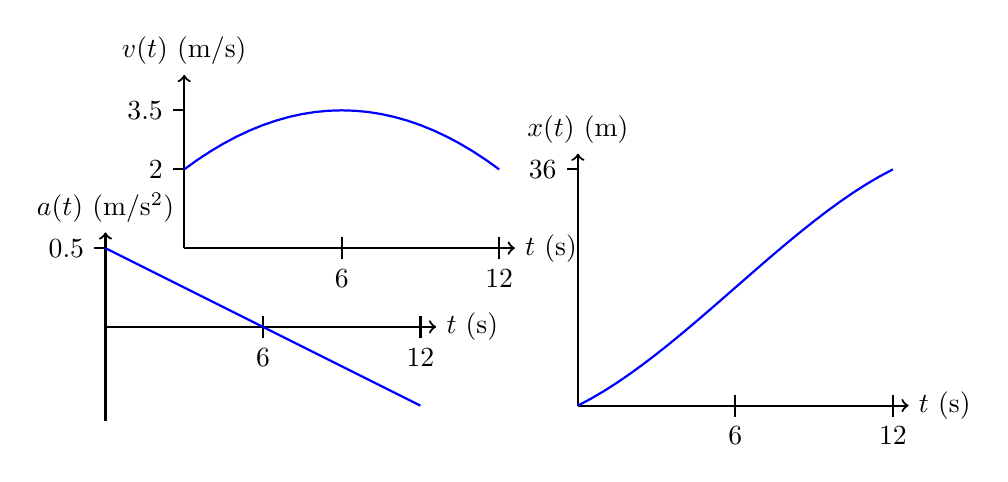
\begin{tikzpicture}
		\begin{scope}
			\draw[thick,->] (0,-1.2) -- (0,1.2) node[anchor=south] {$a(t)$ (m/s$^{2}$)};
			\draw[thick,->] (0,0) -- (4.2,0) node[anchor=west] {$t$ (s)};
			\draw[thick] (2,4pt) -- (2,-4pt) node[anchor=north] {6};
			\draw[thick] (4,4pt) -- (4,-4pt) node[anchor=north] {12};
			\draw[thick] (-4pt,1) node[anchor=east] {0.5} -- (0,1);
			\draw[thick,blue] (0,1) -- (4,-1);
		\end{scope}
		\begin{scope}[shift={(1,1)}]
			\draw[thick,->] (0,0) -- (0,2.2) node[anchor=south] {$v(t)$ (m/s)};
			\draw[thick,->] (0,0) -- (4.2,0) node[anchor=west] {$t$ (s)};
			\draw[thick] (2,4pt) -- (2,-4pt) node[anchor=north] {6};
			\draw[thick] (4,4pt) -- (4,-4pt) node[anchor=north] {12};
			\draw[thick] (-4pt,1) node[anchor=east] {2} -- (0,1);
			\draw[thick] (-4pt,1.75) node[anchor=east] {3.5} -- (0,1.75);
			\draw[thick,blue,domain=0:12,variable=\t] plot (\t/3,{1+0.25*(\t-\t*\t/12)});
		\end{scope}
		\begin{scope}[shift={(6,-1)}]
			\draw[thick,->] (0,0) -- (0,3.2) node[anchor=south] {$x(t)$ (m)};
			\draw[thick,->] (0,0) -- (4.2,0) node[anchor=west] {$t$ (s)};
			\draw[thick] (2,4pt) -- (2,-4pt) node[anchor=north] {6};
			\draw[thick] (4,4pt) -- (4,-4pt) node[anchor=north] {12};
			\draw[thick] (-4pt,3) node[anchor=east] {36} -- (0,3);
			\draw[thick,blue,domain=0:12,variable=\t] plot (\t/3,{(2*\t+0.5*(0.5*\t*\t-\t*\t*\t/36))/12});
		\end{scope}
	\end{tikzpicture}
\end{center}
\end{TeacherMargin}
\begin{PresentSpace}
\vspace{-10pt}
\section*{L4-1: Vax'ildan's Acceleration -- Sensemake}
\vspace{-10pt}
%\begin{multicols}{2}
\begin{itemize}
	\item At $t=0$, Vax clicks his \textit{boots of haste}, which provide an acceleration:
	\[
	\vec{a}(t) = a_{0}\left(1-\frac{t}{T}\right)\hat{x}
	\]
	%\vspace{40pt}
	%\item With your group:
	\item How can we make sense of these equations?
	\begin{align*}
	\vec{v}(t) & = \left[v_{i}+a_{0}\left(t-\frac{t^{2}}{2T}\right)\right]\hat{x} & \vec{x}(t) & = \left[x_{i}+v_{i}t+a_{0}\left(\frac{t^{2}}{2}-\frac{t^{3}}{6T}\right)\right]\hat{x} \\
	t_{f} & = 2T & \vec{x}_{f} & = \left[x_{i}+2v_{i}T+\frac{2}{3}a_{0}T^{2}\right]\hat{x}
	\end{align*}
\end{itemize}
\begin{multicols}{2}
	\begin{itemize}
		\item \textbf{Units}
		\item \textbf{Numbers}
		\begin{itemize}
			\item Which things are vectors?
			\item Try plugging in some reasonable numbers.
		\end{itemize}
		\item \textbf{Symbols}
		\begin{itemize}
			\item What happens if you change $a_{0}$ or $T$?
		\end{itemize}
		\item What do the graphs of $\vec{v}(t)$ and $\vec{a}(t)$ look like?
	\end{itemize}
\end{multicols}
%\end{multicols}
\end{PresentSpace}
%\newpage
\begin{comment}
\noindent\textbf{Calculate}

\noindent\textbf{Represent Principles}

\noindent\textbf{Find Unknowns Symbolically}

\noindent\textbf{Plug in Numbers}

\end{comment}
\begin{comment}
\vspace{-10pt}
\section*{L4-1: Vax'ildan's Acceleration -- Sensemake}
\vspace{-10pt}
\begin{itemize}
	\item How can we make sense of these equations?
	\begin{align*}
		\vec{v}(t) & = \left[v_{i}+a_{0}\left(t-\frac{t^{2}}{2T}\right)\right]\hat{x} & \vec{x}(t) & = \left[x_{i}+v_{i}t+a_{0}\left(\frac{t^{2}}{2}-\frac{t^{3}}{6T}\right)\right]\hat{x} \\
		t_{f} & = 2T & \vec{x}_{f} & = \left[x_{i}+2v_{i}T+\frac{2}{3}a_{0}T^{2}\right]\hat{x}
	\end{align*}
	\begin{itemize}
		\item Are the units correct?
		\item Which things are vectors?
		\item What do the graphs of $\vec{v}(t)$ and $\vec{x}(t)$ look like?
		\item What happens if you change $a_{0}$ or T?
		\item Try plugging in some reasonable numbers: $v_{i} = 2 \text{ m/s},\ T = 8 \text{ s},\ a_{0} = 0.5 \text{ m/s}^{2}, x_{i} = 15 \text{ m}$.
	\end{itemize}
\end{itemize}
\end{comment}
\newpage
\begin{TeacherMargin}
\noindent\textbf{Constant Acceleration} \\
The process for deriving the equations of motion is the same:
\begin{multicols}{2}
	\noindent
	\[
	\begin{split}
		\frac{d\vec{v}}{dt} & = a\hat{x} \\
		d\vec{v} & = adt\hat{x} \\
		\int_{v_{i}}^{v(t)}d\vec{v} & = \int_{0}^{t}adt\hat{x} \\
		\vec{v}(t) - \vec{v}_{i} & = at\hat{x} \\
		\vec{v}(t) & = \left[v_{i}+at\right]\hat{x}
	\end{split}
	\]
	\[
	\begin{split}
		\frac{d\vec{x}}{dt} & = \vec{v}(t) \\
		d\vec{x} & = \vec{v}(t)dt \\
		\int_{x_{i}}^{x(t)}d\vec{x} & = \int_{0}^{t}\left[v_{i}+at\right]dt\hat{x} \\
		\vec{x}(t) - \vec{x}_{i} & = \left[v_{i}t+\frac{1}{2}at^{2}\right]\hat{x} \\
		\vec{x}(t) & = \left[x_{i} + v_{i}t+\frac{1}{2}at^{2}\right]\hat{x}
	\end{split}
	\]
\end{multicols}
These equations are often called the \textbf{kinematics equations}. There is a third kinematics equation often bundled with these that you can derive in Get-Ready \#4 (in \href{https://lipa.physics.oregonstate.edu/sec_kinematics-1d.html}{\color{blue}\S2.15} of the online textbook).
\end{TeacherMargin}
\begin{PresentSpace}
\vspace{-10pt}
\section*{L4-2: Constant Acceleration}
\vspace{-10pt}
\begin{itemize}
	\item What if Vax's acceleration had been constant?
	\[
	\vec{a}(t) = a\hat{x}
	\]
\end{itemize}
\end{PresentSpace}
\newpage
\begin{TeacherMargin}

\end{TeacherMargin}
\begin{PresentSpace}
\section*{Main Ideas}
\begin{itemize}
	\item If we know the acceleration of an object as a function of time, we can determine the velocity as a function of time.
	\item If we know the velocity as a function of time, we can determine the position as a function of time.
\end{itemize}
\end{PresentSpace}
\end{document}